\section{Introduction}
In this chapter, we will lay down the theoretical and computational foundations of our approach for approximating the manifold structure of attributed incentive salience in scenarios where only large volumes of behavioural data are available. First, we will briefly illustrate how previous work has framed the modelling of this construct as a reinforcement learning problem and solved it using Temporal Difference Learning (TD Learning) \cite{sutton1988learning}. This, will provide us with a psycho-biologically plausible computational model of attribute incentive salience and constitute the starting point for our approach. Then, we will highlight how video games are promising candidates for studying the behavioural aspects of incentive salience attribution in naturalistic settings. Finally, combining these two ideas, we will show how estimating the manifold structure of attributed incentive salience can be cast as the solution to a supervised learning problem and why Artificial Neural Networks (ANNs), thanks to their representation learning capabilities, are well suited for the task.

\section{Manifold Representation of Attributed Incentive Salience}
As anticipated in the introduction, we can think of the level of attributed incentive salience (i.e. the amount of \textit{Wanting} attached to a particular object) as a latent state influencing motivated behaviour. The representation of these latent states is usually carried out by the activity of multiple brain regions responsible to generate patterns of observable behaviour. As we mentioned before, these multidimensional patterns are believed to reside on a manifold \cite{seung2000manifold, pang2016dimensionality}: a connected low dimensional region embedded within a high dimensional space \cite{bengio2017deep}. An intuitive example of this is how the brain generates and stores mental maps of the environment which are then used for navigation tasks \cite{derdikman2011manifold, nieh2021geometry}. The dimensionality of the encoding signal is much larger than the intrinsic dimensionality of the spatial information encoded within it, indeed the activity of large neuronal populations is involved in generating a mapping that needs to be only 3 dimensional. When applied to incentive salience an intuitive representation sees the manifold as a 2 dimensional space, similar to what presented in Figure \ref{fig: vect_mot}, generated by the activity of all those brain areas involved in the attribution of value and subsequent modulation of future motivated behaviour. This two dimensional space would represent, at any given time, the motivational saliency than an organism attributes to a potentially rewarding object and therefore also the intensity of the related  behaviour \cite{berridge1998role, simpson2016behavioral}. This idea of a neural manifold has found experimental support in different areas (e.g. motor control \cite{gallego2017neural}, mnemonic processes \cite{derdikman2011manifold, nieh2021geometry}, reward processing \cite{bromberg2010coding} visual \cite{seung2000manifold, ganmor2015thesaurus} and olfactory \cite{stopfer2003intensity} perception) and rely on the fact that neural activity is highly redundant and reducible to just few correlation patterns \cite{gallego2017neural}. In light of this, the use of dimensionality reduction techniques able to represent the manifold structure of highly dimensional data have proven to be valuable in making abstract entities like latent states more easily accessible and interpretable, while also facilitating their mapping onto brain \cite{gao2021nonlinear, rue2021decoding} and behavioural data \cite{luxem2020identifying, pereira2020quantifying, mccullough2021unsupervised, shi2021learning}.

\section{Computational Framework}
\label{comp_framework}
\lorem


\subsection{Temporal Difference Learning}
\label{td_learning}

The first attempt to model incentive salience attribution was carried out by McClure \textit{et. al.} using TD Learning \cite{mcclure2003computational}. The use of TD Learning in simulation studies involving reward learning, is often motivated by its good approximation of the reward-prediction error signal generated by dopaminergic neurons \cite{schultz1997neural,flagel2011selective}. Algorithms in the family of TD Learning attempt to learn a value function $V$ by iteratively refining an estimate $\widehat{V}$ over time \cite{sutton2018reinforcement}. In the most basic form, called TD(0), this is done by simply observing the reward $r$ associated with a particular state $s$ at time $t_{+1}$ and using it to adjust the estimate of $V$ produced at time $t$ \cite{sutton2018reinforcement}. Here $t$ is an arbitrary unit of time, it can be specific (i.e. seconds) or generic (i.e. a point in an ordered series of events) depending on the type of application. If we let $S=\{s_{t}: t \in T\}$ be a sequence of states, then the value $V$  at $s_{t}$ is given by the sum of all future discounted rewards expected when transitioning from $s_t$ to $s_{t+1}$
\begin{align}
\label{td_v}
    V(s_t) 
        &= E[
            r_{t+1} + 
            \gamma r_{t+2} + 
            \gamma^{2} r_{t+3} +
            ... +
            \gamma^{T} r_{T}
        ]\\
        &= E[
            r_{t+1} + 
            \gamma V(s_{t+1}) 
        ] \nonumber
\end{align}
with $\gamma \in [0, 1]$ being a discounting factor for $r$. The iterative refining of $\widehat{V}$ carried out by TD learning is achieved by first computing an error signal $\delta$ at time $t$
\begin{align}
    \label{td_error}
    \delta(t) = r_{t+1} + \gamma \widehat{V}(s_{t+1}) - \widehat{V}(s_{t})
\end{align}
which quantifies the difference between the current $\widehat{V}$ and what is expected when transitioning to $s_{t+1}$. Once the error signal is computed, $\widehat{V}(s_{t})$ is updated as: 
\begin{align}
    \label{td_update}
    \widehat{V}(s_t)  \leftarrow \widehat{V}(s_t) + \alpha(\delta)
\end{align}
where $\alpha \in [0, 1]$ is a constant controlling the amount of updating or the "learning rate". This process called TD update is illustrated by the diagram presented in Figure \ref{fig: td_learning}. Conventionally the transition from $s$ to $s_{t+1}$ is the result of an action selection process guided by $\widehat{V}$, because in optimal control settings the role of reinforcement learning is to select the course of action that maximizes future rewards \cite{schultz1997neural,mcclure2003computational,sutton2018reinforcement}.
\begin{figure}[h]
  \begin{center}
    \begin{adjustbox}{width=0.5\columnwidth}

        \tikzset{every picture/.style={line width=0.75pt}}       
        
        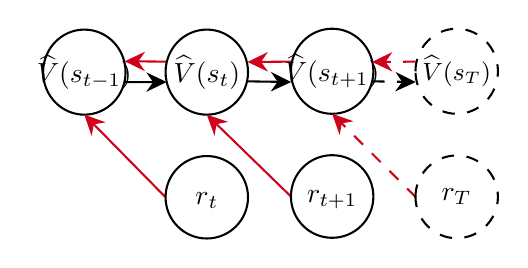
\begin{tikzpicture}[x=0.75pt,y=0.75pt,yscale=-1,xscale=1]
        
        %Straight Lines [id:da2592063600931961] 
        \draw [color={rgb, 255:red, 208; green, 2; blue, 27 }  ,draw opacity=1 ]   (282.5,135.16) -- (300.67,135.02) ;
        \draw [shift={(279.5,135.18)}, rotate = 359.55] [fill={rgb, 255:red, 208; green, 2; blue, 27 }  ,fill opacity=1 ][line width=0.08]  [draw opacity=0] (9.82,-4.72) -- (0,0) -- (9.82,4.72) -- (6.52,0) -- cycle    ;
        %Straight Lines [id:da41585806917853485] 
        \draw [color={rgb, 255:red, 208; green, 2; blue, 27 }  ,draw opacity=1 ]   (223.33,134.87) -- (240.67,135.02) ;
        \draw [shift={(220.33,134.85)}, rotate = 0.47] [fill={rgb, 255:red, 208; green, 2; blue, 27 }  ,fill opacity=1 ][line width=0.08]  [draw opacity=0] (9.82,-4.72) -- (0,0) -- (9.82,4.72) -- (6.52,0) -- cycle    ;
        %Shape: Ellipse [id:dp31493856088290983] 
        \draw   (181,140.07) .. controls (181,128.75) and (189.89,119.58) .. (200.86,119.58) .. controls (211.83,119.58) and (220.72,128.75) .. (220.72,140.07) .. controls (220.72,151.4) and (211.83,160.57) .. (200.86,160.57) .. controls (189.89,160.57) and (181,151.4) .. (181,140.07) -- cycle ;
        %Shape: Ellipse [id:dp5103941395609547] 
        \draw  [dash pattern={on 4.5pt off 4.5pt}] (360.4,139.66) .. controls (360.4,128.34) and (369.29,119.16) .. (380.26,119.16) .. controls (391.23,119.16) and (400.12,128.34) .. (400.12,139.66) .. controls (400.12,150.98) and (391.23,160.16) .. (380.26,160.16) .. controls (369.29,160.16) and (360.4,150.98) .. (360.4,139.66) -- cycle ;
        %Straight Lines [id:da30559831832260953] 
        \draw [color={rgb, 255:red, 0; green, 0; blue, 0 }  ,draw opacity=1 ]   (220.07,144.9) -- (237.5,144.86) ;
        \draw [shift={(240.5,144.85)}, rotate = 539.86] [fill={rgb, 255:red, 0; green, 0; blue, 0 }  ,fill opacity=1 ][line width=0.08]  [draw opacity=0] (9.82,-4.72) -- (0,0) -- (9.82,4.72) -- (6.52,0) -- cycle    ;
        %Shape: Ellipse [id:dp12377292733336898] 
        \draw  [color={rgb, 255:red, 0; green, 0; blue, 0 }  ,draw opacity=1 ] (240,140.07) .. controls (240,128.75) and (248.89,119.58) .. (259.86,119.58) .. controls (270.83,119.58) and (279.72,128.75) .. (279.72,140.07) .. controls (279.72,151.4) and (270.83,160.57) .. (259.86,160.57) .. controls (248.89,160.57) and (240,151.4) .. (240,140.07) -- cycle ;
        %Shape: Ellipse [id:dp9248757796917767] 
        \draw   (300.4,139.66) .. controls (300.4,128.34) and (309.29,119.16) .. (320.26,119.16) .. controls (331.23,119.16) and (340.12,128.34) .. (340.12,139.66) .. controls (340.12,150.98) and (331.23,160.16) .. (320.26,160.16) .. controls (309.29,160.16) and (300.4,150.98) .. (300.4,139.66) -- cycle ;
        %Straight Lines [id:da050274800713848156] 
        \draw [color={rgb, 255:red, 208; green, 2; blue, 27 }  ,draw opacity=1 ]   (202.96,162.71) -- (240,200.37) ;
        \draw [shift={(200.86,160.57)}, rotate = 45.48] [fill={rgb, 255:red, 208; green, 2; blue, 27 }  ,fill opacity=1 ][line width=0.08]  [draw opacity=0] (9.82,-4.72) -- (0,0) -- (9.82,4.72) -- (6.52,0) -- cycle    ;
        %Straight Lines [id:da7059353635730191] 
        \draw [color={rgb, 255:red, 208; green, 2; blue, 27 }  ,draw opacity=1 ]   (262.01,162.66) -- (300.4,200) ;
        \draw [shift={(259.86,160.57)}, rotate = 44.2] [fill={rgb, 255:red, 208; green, 2; blue, 27 }  ,fill opacity=1 ][line width=0.08]  [draw opacity=0] (9.82,-4.72) -- (0,0) -- (9.82,4.72) -- (6.52,0) -- cycle    ;
        %Straight Lines [id:da17885982011746426] 
        \draw [color={rgb, 255:red, 208; green, 2; blue, 27 }  ,draw opacity=1 ] [dash pattern={on 4.5pt off 4.5pt}]  (322.38,162.28) -- (360.4,200.16) ;
        \draw [shift={(320.26,160.16)}, rotate = 44.9] [fill={rgb, 255:red, 208; green, 2; blue, 27 }  ,fill opacity=1 ][line width=0.08]  [draw opacity=0] (9.82,-4.72) -- (0,0) -- (9.82,4.72) -- (6.52,0) -- cycle    ;
        %Shape: Ellipse [id:dp3523005799699832] 
        \draw  [dash pattern={on 4.5pt off 4.5pt}] (360.4,200.16) .. controls (360.4,189.16) and (369.29,180.23) .. (380.26,180.23) .. controls (391.23,180.23) and (400.12,189.16) .. (400.12,200.16) .. controls (400.12,211.17) and (391.23,220.09) .. (380.26,220.09) .. controls (369.29,220.09) and (360.4,211.17) .. (360.4,200.16) -- cycle ;
        %Shape: Ellipse [id:dp3509500153089894] 
        \draw   (300.4,200) .. controls (300.4,189) and (309.29,180.09) .. (320.26,180.09) .. controls (331.23,180.09) and (340.12,189) .. (340.12,200) .. controls (340.12,210.99) and (331.23,219.9) .. (320.26,219.9) .. controls (309.29,219.9) and (300.4,210.99) .. (300.4,200) -- cycle ;
        %Shape: Ellipse [id:dp17336392317383575] 
        \draw  [color={rgb, 255:red, 0; green, 0; blue, 0 }  ,draw opacity=1 ] (240,200.37) .. controls (240,189.4) and (248.89,180.5) .. (259.86,180.5) .. controls (270.83,180.5) and (279.72,189.4) .. (279.72,200.37) .. controls (279.72,211.34) and (270.83,220.23) .. (259.86,220.23) .. controls (248.89,220.23) and (240,211.34) .. (240,200.37) -- cycle ;
        %Straight Lines [id:da21459790152477998] 
        \draw [color={rgb, 255:red, 0; green, 0; blue, 0 }  ,draw opacity=1 ]   (279.5,144.52) -- (297.5,144.8) ;
        \draw [shift={(300.5,144.85)}, rotate = 180.91] [fill={rgb, 255:red, 0; green, 0; blue, 0 }  ,fill opacity=1 ][line width=0.08]  [draw opacity=0] (9.82,-4.72) -- (0,0) -- (9.82,4.72) -- (6.52,0) -- cycle    ;
        %Straight Lines [id:da8588950475203374] 
        \draw [color={rgb, 255:red, 208; green, 2; blue, 27 }  ,draw opacity=1 ] [dash pattern={on 4.5pt off 4.5pt}]  (342.5,135.16) -- (360.67,135.02) ;
        \draw [shift={(339.5,135.18)}, rotate = 359.55] [fill={rgb, 255:red, 208; green, 2; blue, 27 }  ,fill opacity=1 ][line width=0.08]  [draw opacity=0] (9.82,-4.72) -- (0,0) -- (9.82,4.72) -- (6.52,0) -- cycle    ;
        %Straight Lines [id:da9169375689094925] 
        \draw [color={rgb, 255:red, 0; green, 0; blue, 0 }  ,draw opacity=1 ] [dash pattern={on 4.5pt off 4.5pt}]  (339.5,144.52) -- (357.5,144.8) ;
        \draw [shift={(360.5,144.85)}, rotate = 180.91] [fill={rgb, 255:red, 0; green, 0; blue, 0 }  ,fill opacity=1 ][line width=0.08]  [draw opacity=0] (9.82,-4.72) -- (0,0) -- (9.82,4.72) -- (6.52,0) -- cycle    ;
        
        % Text Node
        \draw (320.26,201.59) node    {$r_{t+1}$};
        % Text Node
        \draw (200.86,140.07) node    {$\widehat{V}(s_{t-1})$};
        % Text Node
        \draw (320.26,139.66) node    {$\widehat{V}(s_{t+1})$};
        % Text Node
        \draw (380.26,139.66) node  [font=\small]  {$\widehat{V}(s_{T})$};
        % Text Node
        \draw (259.86,202) node  [color={rgb, 255:red, 208; green, 9; blue, 2 }  ,opacity=1 ]  {$\textcolor[rgb]{0,0,0}{r}\textcolor[rgb]{0,0,0}{_{t}}$};
        % Text Node
        \draw (259.86,140.07) node  [color={rgb, 255:red, 208; green, 9; blue, 2 }  ,opacity=1 ]  {$\textcolor[rgb]{0,0,0}{\widehat{V}}\textcolor[rgb]{0,0,0}{(s_{t})}$};
        % Text Node
        \draw (380.26,200.16) node    {$r_{T}$};

        \end{tikzpicture}
    \end{adjustbox}
  \end{center}
\caption[\textbf{Graphical representation of TD Learning}]{Red arrows indicate the flow of the computations for deriving $\delta$ and updating $\widehat{V}$ expressed by equations \ref{td_error} and \ref{td_update}. Black arrows instead indicate the changes of $\widehat{V}$ moving from $s$ to $s_{t+1}$. Solid circles indicate states which have already been observed while dashed ones represent future not-yet observed states.}
\label{fig: td_learning}
\end{figure}
McClure \textit{et. al.} proposed that incentive salience is represented by $V$ as defined in equation \ref{td_v} while the error signal expressed by equation \ref{td_error} represents the activity of dopaminergic neurons with the dual function of driving the attribution of incentive salience (through reward prediction error coding as specified in section \ref{incentive_salience}) and guiding the previously mentioned action selection process \cite{schultz1997neural,mcclure2003computational,o2003temporal}. However, in later work, Zhang \textit{et. al.} highlighted the fact that the model proposed by McClure \textit{et. al.} fails to take into account an important part of the original incentive salience hypothesis: the dynamic modulation produced by the individual's internal state (see section \ref{wanting}) \cite{toates1994comparing,mcclure2003computational,berridge2004motivation,zhang2009neural,tindell2009dynamic,berridge2012prediction}. Zhang \textit{et. al.} therefore proposed a modification of the original TD Learning model to include a modulatory factor $k \in [0, +\infty]$ which can enhance ($k > 1$), dampen or even revert ($k < 1$) previously learned incentive salience values
\begin{align}
    \label{zhang_td_v}
    V(s_t) = E[\tilde{r}(r_{t+1},k_{t}) + \gamma V(s_{t+1})]
\end{align}
here $\tilde{r}(.,.)$ is a function of two variables and can assume either an additive or multiplicative form \footnote{See \cite{zhang2009neural} for detailed description of the two forms and their functional differences.}. The main difference between the approaches of McClure \textit{et. al.} and Zhang \textit{et. al.} lies in the interpretation of $V$. Both authors see it as a combination of cached value (i.e. what has been learned from past experiences) and expectation over future $r$ but for McClure \textit{et. al.} all the future $r$ have the same weight while for Zhang \textit{et. al.} the state of the individual dynamically modulates the weighting of $r$. Using the notation from section \ref{incentive_salience}, we can say that the interaction $s$ between $I$ and $O$ at time $t_{+1}$ arises from the $V$ (i.e. incentive salience) generated after $s_{t}$. The mismatch between the predicted amount of reward and the actual reward received at time $t_{+1}$ generates an error signal that allows $I$ to learn about the "correct" magnitude of $V(s_{t})$ \cite{schultz2017reward} . As an example, an individual may anticipate that eating their favourite meal would be a rewarding experience but instead (for some reason) it was underwhelming. They therefore reduce the salience previously attributed to it. Importantly, $V(s_{t})$ does not just encompass the previous history of interactions between $I$ and $O$ but also the current state of $I$: the individual has learned from long experience that eating is a pleasurable activity but currently, since they are sated they do not expect much reward from doing it again in the near future.  

\paragraph{\textbf{From TD to Supervised Learning}}
\label{td_to_supervised}
The approaches discussed above frame the estimation of attributed incentive salience as a reinforcement learning task. This requires the simulation of a sequence of interactions between $I$ and $O$ and the concomitant delivery of $r$  \cite{schultz1997neural,mcclure2003computational,zhang2009neural}. However, it is not always straightforward to replicate these interactions in real world scenarios, especially when dealing with human participants. The control on the internal state of $I$ and amount of $r$ delivered that McClure and Zhang assume is usually based on strict assumptions and can be achieved only in controlled experimental settings \cite{mcclure2003computational,zhang2009neural}. As an alternative solution for inferring $V$ outside the laboratory we propose to learn its manifold structure through supervised learning. Differently to what reported in the literature \cite{calhoun2019unsupervised, mccullough2021unsupervised, luxem2020identifying, pereira2020quantifying, shi2021learning} we argue that in this case the use of supervised in place of un-supervised techniques is to be preferred. Indeed, since we are dealing exclusively with behavioural data and trying to solve an inverse problem  we would like to learn a manifold structure which is not just a generic indicator of behavioural phenotype \cite{luxem2020identifying} but also obeys to specific functional constrains.\\
\\
In this approach, an experimenter gathers data on a set of interactions between $I$ and $O$ and let a learning algorithm to estimate two functions:
\begin{gather}
\label{supervised_v}
    V(s_{t}) = f^{1}(O, \tilde{r_{t}}, V(s_{t-1}); \theta^{1}) \\
    r_{t+1} = f^{2}(V(s_{t}); \theta^{2}) \nonumber
\end{gather}
here $f^{1}$ and $f^{2}$ are arbitrarily complex functions while $\theta^{1}$ and $\theta^{2}$ are parameters that the learning algorithm has to infer. The future reward that an individual expects after an interaction with an object is produced by the current level of attributed salience, which  itself is a function of the current internal state of the individual (expressed through the amount of reward just experienced) and the incentive salience previously attributed to the object. It is important to note that the two functions above need to be recursive over all $s \in S$ (see equations \ref{td_v} and \ref{zhang_td_v}) in order to provide $V(s_{t})$ with the dual purpose of caching all the past $V$ and being a suitable predictor for all the $r$. This formulation however still requires a measure of the $r$ experienced by $I$ (or more precisely its weighted version $\tilde{r}$) after interacting with $O$, which is not easily accessible. However, Thorndike's law of effect \cite{thorndike1927law} and Skinner's operant conditioning principles \cite{skinner1965science} suggest that $r$, which  like $V$ is a non observable latent variable, manifests itself through the intensity of interactions between $I$ and $O$ (i.e. $B$ in Figure \ref{fig: incs} and section \ref{motivation}): the frequency and amount of object-directed behaviours increase or decrease as a function of the rewards an individual expects to receive \cite{berridge2004motivation,schultz2017reward}. Since $V(s_{t})$ predicts how much $r$ an $I$ expects to receive from interacting with $O$, we should also expect the strength of their future interactions to be a function of $V(s_{t})$. This can be represented re-arranging the equations in \ref{supervised_v} in a more compact form as a chain of functions
\begin{align}
\label{supervised_b}
    B_{t+1} = f^{2}(f^{1}(O, B_{t}, V(s_{t-1}); \theta^{1});  \theta^{2})
\end{align}
To approximate the above expression, a learning algorithm would require records of behaviours generated by individuals while interacting with a diverse set of potentially rewarding objects. Here, we argue that video games are one way to obtain this type of data at scale while also achieving some level of ecological validity.

\subsection{Video Games and Telemetry}
\label{videogame_telemetries}
Interacting with video games is a volitional activity driven largely by the capacity of the games to provide pleasurable experiences \cite{boyle2012engagement}. Behaviour within the game is best understood as the result of a value attribution process similar to that of secondary reward objects (see section \ref{incentive_salience}). Indeed, it appears that the play behaviour is often produced and maintained by the structural characteristics of the game (e.g. game mechanics) \cite{king2010video} which, working like conventional reinforcement mechanisms \cite{chumbley2006affect,wang2011game,phillips2013videogame,avserivskis2017computational}, produce effects similar to operant conditioning \cite{skinner1965science}. Although caution should be applied when complex activities are investigated using neuroimaging techniques, evidence suggest that the maintenance of video games playing behaviour engages the same cortico-striatal structures \cite{hoeft2008gender,mathiak2011reward,cole2012interactivity,klasen2012neural,lorenz2015video,gleich2017functional} and neurotransmitters \cite{koepp1998evidence} involved in reward processing. This, seems also supported at the behavioural level where the ammount of experienced in-game reward appears to play a role in controlling how likely is an individual to keep engaging in playing behaviour \cite{agarwal2017quitting, steyvers2019joint}. This, in conjunction with a growing literature highlighting similarities between certain video game mechanics and activities driven by secondary rewards (e.g. gambling) \cite{king2010role,drummond2018video,zendle2018video}, corroborates the idea that video games are able to elicit behavioural responses through incentive mechanics. In this view, video games with different structural characteristics could be seen as objects possessing rewarding properties that heavily depend on the individuals interacting with them (e.g. an individual's preference for a specific game mechanic). Hence, similarly to the process specified in section \ref{theoretical_framework}, we can expect that through repeated interactions, an individual will experience varying degrees of reward determined by their internal state and the characteristics of the game. These interactions will produce continuous adjustments in the level of saliency attributed to playing that specific game which in turn will influence the frequency and amount of future interactions with that same game. Other than offering a context for observing the process of incentive salience attribution, video games allow us to obtain large volumes of behavioural data (similar to those mentioned in section \ref{td_to_supervised}) in a naturalistic fashion. This is made possible by the widespread practice of obtaining high frequency records (i.e. telemetry\footnote{See \cite{el2016game} for a more technical description of telemetry in video games.}) of players' behaviour during the game \cite{drachen2015behavioral}. This approach, despite offering less control and rigour than conventional experimental procedures, allows us to obtain a more faithful representation of natural behaviour (similarly to field studies) while avoiding some of the limitations connected with laboratory-based studies (e.g. sampling and observer biases).
\newline
\newline
In order to use this type of behavioural data to model attributed incentive salience, a learning algorithm should possess the following properties. First, it should be scalable and noise resilient, to leverage large volumes of naturalistic data in an efficient and effective manner. Second, it should be able to approximate arbitrarily complex functions, given that the shape of the functions specified in equation \ref{td_to_supervised} is not known a-priori. And finally, it should be able to produce an approximation of $V(s_{t})$ that can be inspected in order to evaluate if its functional properties can be compared with those of attributed incentive salience. Artificial Neural Networks (ANNs) appear to satisfy these requirements.

\subsection{Artificial Neural Networks}
\label{artificial_neural_networks}
In their conventional form, ANNs can be seen as chains of nested functions (the layers of the network). These layers are vector valued (there are multiple units or neurons in each layer) and organized as directed acyclic computational graphs (information only flows forward). When the number of layers is greater than two, the prefix "deep" is usually applied \cite{bengio2017deep}. The goal of this ensemble of functions is to create a mapping between an input $x$ and a target $y$. Following the example illustrated in Figure \ref{fig: ffnn}, given the set of parameters $\Theta = \{\theta^1, \theta^2 \}$ an ANN would first infer a function $h = f(x;\theta^{1})$, mapping the input to a new representation $h$. The same representation $h$ would then become the input of a second function $\widehat{y} = f^{1}(h;\theta^{2})$ which produces an estimate of the target \cite{bengio2017deep}. In this sense, we can think of each layer as a collection of many non-linear vector to scalar functions taking the previous layer as input and generating the units for the layer that follows \cite{bengio2017deep}. By increasing the number of layers and units, ANNs can approximate an extremely large class of functions \cite{rumelhart1986learning}.
\begin{figure}
    \begin{center}
        \begin{adjustbox}{width=0.4\textwidth}
            \tikzset{every picture/.style={line width=0.75pt}} %set default line width to 0.75pt        
            
            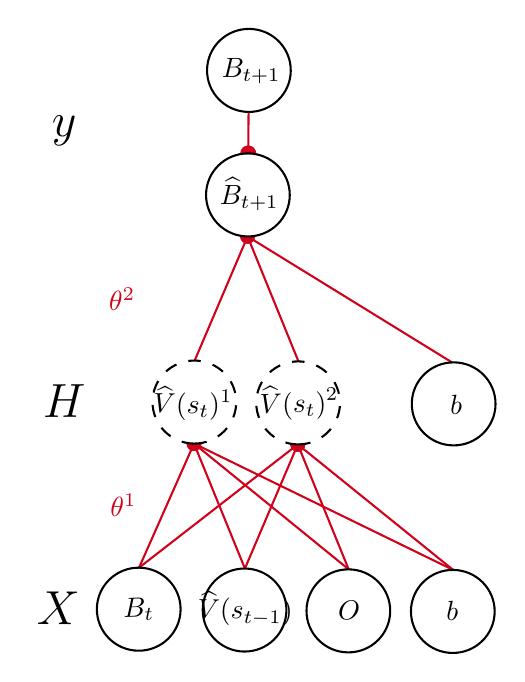
\begin{tikzpicture}[x=0.75pt,y=0.75pt,yscale=-1,xscale=1]
            %uncomment if require: \path (0,350); %set diagram left start at 0, and has height of 350
            
            %Straight Lines [id:da8866607252953388] 
            \draw [color={rgb, 255:red, 208; green, 2; blue, 27 }  ,draw opacity=1 ]   (227.88,279.44) -- (254.36,219.65) ;
            \draw [shift={(254.36,219.65)}, rotate = 293.89] [color={rgb, 255:red, 208; green, 2; blue, 27 }  ,draw opacity=1 ][fill={rgb, 255:red, 208; green, 2; blue, 27 }  ,fill opacity=1 ][line width=0.75]      (0, 0) circle [x radius= 3.02, y radius= 3.02]   ;
            %Straight Lines [id:da0731191645042184] 
            \draw [color={rgb, 255:red, 208; green, 2; blue, 27 }  ,draw opacity=1 ]   (254.68,179.65) -- (280.16,119.85) ;
            \draw [shift={(280.16,119.85)}, rotate = 293.08] [color={rgb, 255:red, 208; green, 2; blue, 27 }  ,draw opacity=1 ][fill={rgb, 255:red, 208; green, 2; blue, 27 }  ,fill opacity=1 ][line width=0.75]      (0, 0) circle [x radius= 3.02, y radius= 3.02]   ;
            %Straight Lines [id:da4826752085294559] 
            \draw [color={rgb, 255:red, 208; green, 2; blue, 27 }  ,draw opacity=1 ]   (304.68,180.05) -- (280.16,119.85) ;
            \draw [shift={(280.16,119.85)}, rotate = 247.84] [color={rgb, 255:red, 208; green, 2; blue, 27 }  ,draw opacity=1 ][fill={rgb, 255:red, 208; green, 2; blue, 27 }  ,fill opacity=1 ][line width=0.75]      (0, 0) circle [x radius= 2.01, y radius= 2.01]   ;
            %Straight Lines [id:da39539248901414714] 
            \draw [color={rgb, 255:red, 208; green, 2; blue, 27 }  ,draw opacity=1 ]   (328.88,280.25) -- (304.36,220.05) ;
            \draw [shift={(304.36,220.05)}, rotate = 247.84] [color={rgb, 255:red, 208; green, 2; blue, 27 }  ,draw opacity=1 ][fill={rgb, 255:red, 208; green, 2; blue, 27 }  ,fill opacity=1 ][line width=0.75]      (0, 0) circle [x radius= 3.02, y radius= 3.02]   ;
            %Straight Lines [id:da8990891706173756] 
            \draw [color={rgb, 255:red, 208; green, 2; blue, 27 }  ,draw opacity=1 ]   (278.88,279.85) -- (254.36,219.65) ;
            \draw [shift={(254.36,219.65)}, rotate = 247.84] [color={rgb, 255:red, 208; green, 2; blue, 27 }  ,draw opacity=1 ][fill={rgb, 255:red, 208; green, 2; blue, 27 }  ,fill opacity=1 ][line width=0.75]      (0, 0) circle [x radius= 3.02, y radius= 3.02]   ;
            %Straight Lines [id:da1147021220204143] 
            \draw [color={rgb, 255:red, 208; green, 2; blue, 27 }  ,draw opacity=1 ]   (328.88,280.25) -- (254.36,219.65) ;
            \draw [shift={(254.36,219.65)}, rotate = 219.12] [color={rgb, 255:red, 208; green, 2; blue, 27 }  ,draw opacity=1 ][fill={rgb, 255:red, 208; green, 2; blue, 27 }  ,fill opacity=1 ][line width=0.75]      (0, 0) circle [x radius= 3.02, y radius= 3.02]   ;
            %Straight Lines [id:da30405558125224674] 
            \draw [color={rgb, 255:red, 208; green, 2; blue, 27 }  ,draw opacity=1 ]   (278.88,279.85) -- (304.36,220.05) ;
            \draw [shift={(304.36,220.05)}, rotate = 293.08] [color={rgb, 255:red, 208; green, 2; blue, 27 }  ,draw opacity=1 ][fill={rgb, 255:red, 208; green, 2; blue, 27 }  ,fill opacity=1 ][line width=0.75]      (0, 0) circle [x radius= 3.02, y radius= 3.02]   ;
            %Straight Lines [id:da7841365763851936] 
            \draw [color={rgb, 255:red, 208; green, 2; blue, 27 }  ,draw opacity=1 ]   (227.88,279.44) -- (304.36,220.05) ;
            \draw [shift={(304.36,220.05)}, rotate = 322.17] [color={rgb, 255:red, 208; green, 2; blue, 27 }  ,draw opacity=1 ][fill={rgb, 255:red, 208; green, 2; blue, 27 }  ,fill opacity=1 ][line width=0.75]      (0, 0) circle [x radius= 3.02, y radius= 3.02]   ;
            %Straight Lines [id:da5618158283475858] 
            \draw [color={rgb, 255:red, 208; green, 2; blue, 27 }  ,draw opacity=1 ]   (379.21,280.52) -- (304.36,220.05) ;
            \draw [shift={(304.36,220.05)}, rotate = 218.93] [color={rgb, 255:red, 208; green, 2; blue, 27 }  ,draw opacity=1 ][fill={rgb, 255:red, 208; green, 2; blue, 27 }  ,fill opacity=1 ][line width=0.75]      (0, 0) circle [x radius= 3.02, y radius= 3.02]   ;
            %Straight Lines [id:da4509011415852858] 
            \draw [color={rgb, 255:red, 208; green, 2; blue, 27 }  ,draw opacity=1 ]   (378.61,180.51) -- (280.16,119.85) ;
            \draw [shift={(280.16,119.85)}, rotate = 211.64] [color={rgb, 255:red, 208; green, 2; blue, 27 }  ,draw opacity=1 ][fill={rgb, 255:red, 208; green, 2; blue, 27 }  ,fill opacity=1 ][line width=0.75]      (0, 0) circle [x radius= 3.02, y radius= 3.02]   ;
            %Straight Lines [id:da7242656967921071] 
            \draw [color={rgb, 255:red, 208; green, 2; blue, 27 }  ,draw opacity=1 ]   (379.21,280.52) -- (254.36,219.65) ;
            \draw [shift={(254.36,219.65)}, rotate = 205.99] [color={rgb, 255:red, 208; green, 2; blue, 27 }  ,draw opacity=1 ][fill={rgb, 255:red, 208; green, 2; blue, 27 }  ,fill opacity=1 ][line width=0.75]      (0, 0) circle [x radius= 3.02, y radius= 3.02]   ;
            %Shape: Ellipse [id:dp9097533963365589] 
            \draw  [fill={rgb, 255:red, 255; green, 255; blue, 255 }  ,fill opacity=1 ][dash pattern={on 4.5pt off 4.5pt}] (304.36,220.05) .. controls (293.22,219.96) and (284.26,210.94) .. (284.35,199.89) .. controls (284.44,188.84) and (293.54,179.96) .. (304.68,180.05) .. controls (315.82,180.14) and (324.77,189.17) .. (324.69,200.21) .. controls (324.6,211.26) and (315.5,220.14) .. (304.36,220.05) -- cycle ;
            %Shape: Ellipse [id:dp9467435778420286] 
            \draw  [fill={rgb, 255:red, 255; green, 255; blue, 255 }  ,fill opacity=1 ][dash pattern={on 4.5pt off 4.5pt}] (254.36,219.65) .. controls (243.22,219.56) and (234.27,210.53) .. (234.36,199.49) .. controls (234.44,188.44) and (243.54,179.56) .. (254.68,179.65) .. controls (265.82,179.74) and (274.78,188.77) .. (274.69,199.81) .. controls (274.6,210.86) and (265.5,219.74) .. (254.36,219.65) -- cycle ;
            %Shape: Ellipse [id:dp4514100854948462] 
            \draw  [fill={rgb, 255:red, 255; green, 255; blue, 255 }  ,fill opacity=1 ] (379.29,220.52) .. controls (368.15,220.43) and (359.2,211.4) .. (359.29,200.36) .. controls (359.37,189.31) and (368.47,180.43) .. (379.61,180.52) .. controls (390.75,180.61) and (399.71,189.64) .. (399.62,200.68) .. controls (399.53,211.73) and (390.43,220.61) .. (379.29,220.52) -- cycle ;
            %Shape: Ellipse [id:dp2836578028815524] 
            \draw  [fill={rgb, 255:red, 255; green, 255; blue, 255 }  ,fill opacity=1 ] (227.56,319.44) .. controls (216.42,319.35) and (207.46,310.32) .. (207.55,299.28) .. controls (207.64,288.23) and (216.74,279.35) .. (227.88,279.44) .. controls (239.02,279.53) and (247.97,288.56) .. (247.89,299.6) .. controls (247.8,310.65) and (238.7,319.53) .. (227.56,319.44) -- cycle ;
            %Shape: Ellipse [id:dp10987171532240936] 
            \draw  [fill={rgb, 255:red, 255; green, 255; blue, 255 }  ,fill opacity=1 ] (278.56,319.85) .. controls (267.42,319.76) and (258.46,310.73) .. (258.55,299.69) .. controls (258.64,288.64) and (267.74,279.76) .. (278.88,279.85) .. controls (290.02,279.94) and (298.97,288.96) .. (298.88,300.01) .. controls (298.79,311.06) and (289.69,319.94) .. (278.56,319.85) -- cycle ;
            %Shape: Ellipse [id:dp5734471221931936] 
            \draw  [fill={rgb, 255:red, 255; green, 255; blue, 255 }  ,fill opacity=1 ] (328.56,320.25) .. controls (317.42,320.16) and (308.46,311.13) .. (308.55,300.09) .. controls (308.64,289.04) and (317.74,280.16) .. (328.88,280.25) .. controls (340.01,280.34) and (348.97,289.37) .. (348.88,300.41) .. controls (348.79,311.46) and (339.69,320.34) .. (328.56,320.25) -- cycle ;
            %Shape: Ellipse [id:dp8405299754625457] 
            \draw  [fill={rgb, 255:red, 255; green, 255; blue, 255 }  ,fill opacity=1 ] (378.89,320.52) .. controls (367.75,320.43) and (358.79,311.4) .. (358.88,300.36) .. controls (358.97,289.31) and (368.07,280.43) .. (379.21,280.52) .. controls (390.35,280.61) and (399.3,289.64) .. (399.21,300.68) .. controls (399.13,311.73) and (390.03,320.61) .. (378.89,320.52) -- cycle ;
            %Straight Lines [id:da531681756338569] 
            \draw [color={rgb, 255:red, 208; green, 2; blue, 27 }  ,draw opacity=1 ]   (280.48,79.86) -- (280.64,59.86) ;
            \draw [shift={(280.48,79.86)}, rotate = 270.46] [color={rgb, 255:red, 208; green, 2; blue, 27 }  ,draw opacity=1 ][fill={rgb, 255:red, 208; green, 2; blue, 27 }  ,fill opacity=1 ][line width=0.75]      (0, 0) circle [x radius= 3.35, y radius= 3.35]   ;
            %Shape: Ellipse [id:dp7122318662628844] 
            \draw  [fill={rgb, 255:red, 255; green, 255; blue, 255 }  ,fill opacity=1 ] (280.64,59.86) .. controls (269.51,59.77) and (260.55,50.74) .. (260.64,39.69) .. controls (260.73,28.65) and (269.83,19.77) .. (280.97,19.86) .. controls (292.1,19.95) and (301.06,28.97) .. (300.97,40.02) .. controls (300.88,51.06) and (291.78,59.95) .. (280.64,59.86) -- cycle ;
            %Shape: Ellipse [id:dp8923679098088735] 
            \draw  [fill={rgb, 255:red, 255; green, 255; blue, 255 }  ,fill opacity=1 ] (280.16,119.85) .. controls (269.03,119.76) and (260.07,110.74) .. (260.16,99.69) .. controls (260.25,88.65) and (269.35,79.77) .. (280.48,79.86) .. controls (291.62,79.94) and (300.58,88.97) .. (300.49,100.02) .. controls (300.4,111.06) and (291.3,119.94) .. (280.16,119.85) -- cycle ;
            
            % Text Node
            \draw (279.05,299.33) node  [rotate=-0.94] [align=left] {$\displaystyle \widehat{V}(s_{t-1})$};
            % Text Node
            \draw (329.04,300.22) node  [rotate=-1.88] [align=left] {$\displaystyle O$};
            % Text Node
            \draw (378.8,300.47) node  [rotate=-359.63] [align=left] {$\displaystyle b$};
            % Text Node
            \draw (380.6,200.87) node  [rotate=-358.65] [align=left] {$\displaystyle b$};
            % Text Node
            \draw (253.92,200.36) node  [rotate=-0.88] [align=left] {$\displaystyle \widehat{V}(s_{t})^1$};
            % Text Node
            \draw (305.05,199.96) node  [rotate=-358.47] [align=left] {$\displaystyle \widehat{V}(s_{t})^2$};
            % Text Node
            \draw (280.95,99.59) node  [rotate=-359.67] [align=left] {$\displaystyle \widehat{B}_{t+1}$};
            % Text Node
            \draw (189,299.2) node  [font=\LARGE,rotate=-0.33]  {$X$};
            % Text Node
            \draw (191.8,199.22) node  [font=\LARGE,rotate=-359.71]  {$H$};
            % Text Node
            \draw (191.84,69.22) node  [font=\LARGE,rotate=-0.13]  {$y$};
            % Text Node
            \draw (220.4,249.43) node  [font=\normalsize,color={rgb, 255:red, 0; green, 0; blue, 0 }  ,opacity=1 ,rotate=-359.94]  {$\textcolor[rgb]{0.82,0.01,0.11}{\theta }\textcolor[rgb]{0.82,0.01,0.11}{^{1}}$};
            % Text Node
            \draw (219.7,149.93) node  [font=\normalsize,color={rgb, 255:red, 208; green, 2; blue, 27 }  ,opacity=1 ,rotate=-359.3]  {$\textcolor[rgb]{0.82,0.01,0.11}{\theta }\textcolor[rgb]{0.82,0.01,0.11}{^{2}}$};
            % Text Node
            \draw (227.72,299.44) node  [rotate=-358] [align=left] {$\displaystyle B_{t}$};
            % Text Node
            \draw (281.85,40.31) node  [rotate=-359.39] [align=left] {$\displaystyle B_{t+1}$};
            
            
            \end{tikzpicture}
        \end{adjustbox}
    \end{center}
\caption[\textbf{Feedforward ANN with a 2-units hidden layer}]{The figure represents how a feedforward ANN could be used for estimating $V(s_t)$ given a sequence of observed behaviors ($B$) produced while interacting with an object ($O$). Here $X$ and $H$ indicates the model's input and the inferred representation.  $y$ indicates both the target and the estimate produced by the model while $b$ is a bias term. The collection of all the red lines indicates the $\Theta$ that the ANN has to estimate while each line represents a single parameter $w$ or $b$. The circles are computational units (i.e. artificial neurons) whose outputs are given by $\phi(W_i^ \top X+ b )$. Here, $\phi$ is a non-linear function conventionally called activation, $W_i$ the weight matrix for the $i^{th}$ unit, $b$ the bias vector and $X$ the output from the previous layer.}
\label{fig: ffnn}
\end{figure}
An ANN finds the optimal values for $\Theta$ by taking forward and a backward passes through the computational graph. In the forward pass, information flows from the input $x$ to the estimate $\widehat{y}$ according to the operations specified in Figure \ref{fig: ffnn}. During the backward pass, the error between $\widehat{y}$ and the target is first computed
\begin{gather}
\label{loss}
    E =  L(y, \widehat{y})
\end{gather}
Here $L$ is a generic convex and differentiable function measuring the distance between $y$ and $\widehat{y}$. Then, the gradient of the error with respect to all the parameters is found and an update is performed taking steps of size $\alpha \in [0, 1]$ in the direction opposite to the gradient
\begin{gather}
\label{delta_rule}
    \Delta w^{j}_{i} = -\alpha\frac{\partial E}{\partial w^{j}_{i}} \\
    w^{j}_{i} \leftarrow w^{j}_{i} + \Delta w^{j}_{i} \nonumber
\end{gather}
What we illustrated here is the application of the delta rule for updating the $i^{th}$ parameter of the $j^{th}$ layer through gradient descent \cite{widrow1960adaptive}. Deep feedforward ANNs rely on a generalization of this rule (i.e. backpropagation \cite{rumelhart1986learning}) for efficiently computing the gradient for all the parameters in the network.  
\\
\\
Returning to the supervised learning problem specified in section \ref{td_to_supervised}, a feedforward ANN approximates $V(s_{t})$ by mapping the inputs of equation \ref{supervised_b} to a candidate $\widehat{V}(s_{t})$ which is then used to generate an estimate $\widehat{B}_{t+1}$. Then, during the backward pass $\widehat{V}(s_{t})$ is adjusted based on the degree of mismatch between the estimation that it produced and the real value of $B_{t+1}$. It is of interest to note that there is a certain degree of overlap between how ANNs adjust their weights and the TD update illustrated in section \ref{td_learning}. Indeed, in single-step scenarios (i.e. predicting $s_{t+1}$ based on $s_{t}$ for each $s \in S$) the parameter changes produced by the two methods are the same \cite{sutton1988learning}. The major difference lies in the delivery of the update: TD learning performs it at every step while backpropagation-based algorithms must  wait until the end of the sequence in order to collate all the observed errors in a single term \cite{sutton1988learning}.

\paragraph{\textbf{Recurrent Neural Networks}}
\label{rnn_theory}
Despite their universal function approximation properties \cite{hornik1989multilayer}, feedforward ANNs are not suitable for the type of recursive operations expressed in paragraph \ref{td_to_supervised} \cite{bengio2017deep}. As we can see from Figure \ref{fig: ffnn_rnn}A, given a sequence of inputs and targets, a conventional feedforward ANN would be limited to learning a temporally local function of the form
\begin{gather}
\label{td_ffnn}
    B_{t+1} = f^2(f^1(O, B_{t}; \theta^{1}); \theta^{2})
\end{gather}
Even when $\Theta$ are shared across time, the estimated $\widehat{V}(s_t)$ cannot incorporate information from past $\widehat{V}(s)$ nor guarantee predictive power for the future $B$. A solution to this problem is offered by ANNs with feedback connections like Recurrent Neural Networks (RNNs). These  are a class of ANNs that are able to efficiently process long sequences of data while also relaxing the requirements of conventional feedforward ANNs for fixed length inputs \cite{bengio2017deep}. Looking at Figure \ref{fig: ffnn_rnn}B, we see that for each $t \in T$ a RNN would compute $\widehat{V}(s_t)$ using both the input $OB_{t}$ and the previously estimated representation $\widehat{V}(s_{t-1})$. This, in combination with the recursive application of $\Theta$, allows the network to learn a function over the entire temporal sequence and to provide $\widehat{V}(s_t)$ with the desirable properties mentioned in section \ref{td_to_supervised}. The structure of $\Theta$ is more complex in RNNs than in feedforward ANNs \footnote{See \cite{bengio2017deep} for a description of the parameters' structure in RNNs.} and a detailed derivation of the underlying optimization process is outside the scope of the present work. Nevertheless, it is worth singling out how the recurrent nature of the computations underlying the generation of $\widehat{V}(s_t)$  makes RNNs suitable for approximating the function specified in section \ref{td_to_supervised}. \\
\\
Following Figure \ref{fig: ffnn_rnn}B, let $\widehat{V}(s_t)$ be the representation inferred by the model at time $t$ and its associated parameters. Optimal parameter values are found through the same update rule used in feedforward ANNs
\begin{gather}
\label{bptt_1}
    \widehat{V}(s_t) \leftarrow \widehat{V}(s_t) + -\alpha \frac{\partial E}{\partial \widehat{V}(s_t)}
\end{gather}
however, since $E$ can now only be observed at the end of a temporal sequence, computing $\frac{\partial E}{\partial \widehat{V}(s_t)}$ requires us to take into account all the intermediate steps from $t$ to $T$. This is achieved applying the chain rule and propagating the error gradient backward in time \cite{bengio2017deep,lillicrap2019backpropagation}
\begin{gather}
\label{bptt_2}
    \frac{\partial E}{\partial \widehat{V}(s_t)} = 
    \frac{\partial E}{\partial \widehat{V}(s_{T})}
    \frac{\partial \widehat{V}(s_{T})}{\partial \widehat{V}(s_{T-1})}
    \dots
    \frac{\partial \widehat{V}(s_{T-n})}{\partial \widehat{V}(s_{t})}
\end{gather}
This implies that, similarly to TD update, the error flow forces $\widehat{V}(s_t)$ to retain information from $OB_t$ and $\widehat{V}(s_{t-1})$ in order to perform estimation of $B_{t+1}$ while still being useful for generating $\widehat{V}(s_{t+1})$ as we can see from Figure \ref{fig: ffnn_rnn}B. This process is made more efficient by an RNN variant called Long Short-Term Memory (LSTM) \cite{hochreiter1997long}, which, as well as improving the propagation of the error gradient, has specialized mechanisms for inferring, at each point in time, which portion of information should be kept or discarded in order to minimize $E$ \cite{hochreiter1997long,bengio2017deep}.
\begin{figure}[h]
\begin{center}
\begin{adjustbox}{width=0.5\columnwidth}
    \tikzset{every picture/.style={line width=0.75pt}} %set default line width to 0.75pt        
    
    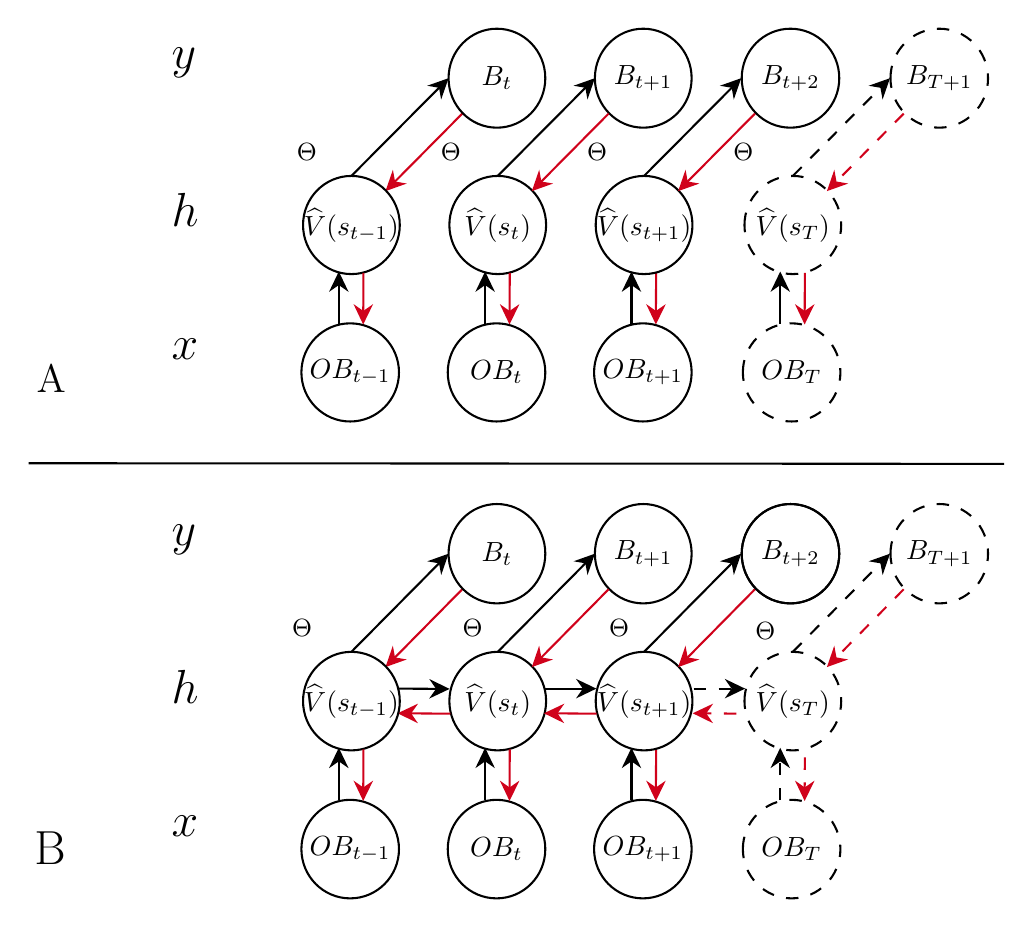
\begin{tikzpicture}[x=0.75pt,y=0.75pt,yscale=-1,xscale=1]
    %uncomment if require: \path (0,432); %set diagram left start at 0, and has height of 432
    
    %Shape: Ellipse [id:dp9152556376471453] 
    \draw   (252.87,325.26) .. controls (252.87,312.15) and (263.3,301.52) .. (276.18,301.52) .. controls (289.05,301.52) and (299.48,312.15) .. (299.48,325.26) .. controls (299.48,338.37) and (289.05,349) .. (276.18,349) .. controls (263.3,349) and (252.87,338.37) .. (252.87,325.26) -- cycle ;
    %Straight Lines [id:da0084456304461753] 
    \draw [color={rgb, 255:red, 208; green, 2; blue, 27 }  ,draw opacity=1 ]   (230.94,331.15) -- (253.32,331.31) ;
    \draw [shift={(227.94,331.12)}, rotate = 0.43] [fill={rgb, 255:red, 208; green, 2; blue, 27 }  ,fill opacity=1 ][line width=0.08]  [draw opacity=0] (9.82,-4.72) -- (0,0) -- (9.82,4.72) -- (6.52,0) -- cycle    ;
    %Shape: Ellipse [id:dp18326344407352502] 
    \draw   (181.58,396.56) .. controls (181.58,383.45) and (192.11,372.82) .. (205.08,372.82) .. controls (218.06,372.82) and (228.59,383.45) .. (228.59,396.56) .. controls (228.59,409.67) and (218.06,420.3) .. (205.08,420.3) .. controls (192.11,420.3) and (181.58,409.67) .. (181.58,396.56) -- cycle ;
    %Shape: Ellipse [id:dp4732045107682973] 
    \draw   (252.09,396.56) .. controls (252.09,383.45) and (262.61,372.82) .. (275.59,372.82) .. controls (288.57,372.82) and (299.09,383.45) .. (299.09,396.56) .. controls (299.09,409.67) and (288.57,420.3) .. (275.59,420.3) .. controls (262.61,420.3) and (252.09,409.67) .. (252.09,396.56) -- cycle ;
    %Straight Lines [id:da9106304988340169] 
    \draw    (205.67,301.52) -- (250.37,256.37) ;
    \draw [shift={(252.48,254.24)}, rotate = 494.71] [fill={rgb, 255:red, 0; green, 0; blue, 0 }  ][line width=0.08]  [draw opacity=0] (9.82,-4.72) -- (0,0) -- (9.82,4.72) -- (6.52,0) -- cycle    ;
    %Straight Lines [id:da5186602107869037] 
    \draw [color={rgb, 255:red, 208; green, 2; blue, 27 }  ,draw opacity=1 ]   (259.09,271.36) -- (224.2,306.73) ;
    \draw [shift={(222.1,308.86)}, rotate = 314.62] [fill={rgb, 255:red, 208; green, 2; blue, 27 }  ,fill opacity=1 ][line width=0.08]  [draw opacity=0] (9.82,-4.72) -- (0,0) -- (9.82,4.72) -- (6.52,0) -- cycle    ;
    %Shape: Ellipse [id:dp6434768624828036] 
    \draw   (322.59,396.56) .. controls (322.59,383.45) and (333.11,372.82) .. (346.09,372.82) .. controls (359.07,372.82) and (369.59,383.45) .. (369.59,396.56) .. controls (369.59,409.67) and (359.07,420.3) .. (346.09,420.3) .. controls (333.11,420.3) and (322.59,409.67) .. (322.59,396.56) -- cycle ;
    %Shape: Ellipse [id:dp4847846412537088] 
    \draw   (252.48,254.24) .. controls (252.48,241.02) and (262.91,230.3) .. (275.78,230.3) .. controls (288.65,230.3) and (299.09,241.02) .. (299.09,254.24) .. controls (299.09,267.46) and (288.65,278.18) .. (275.78,278.18) .. controls (262.91,278.18) and (252.48,267.46) .. (252.48,254.24) -- cycle ;
    %Shape: Ellipse [id:dp07973567399208026] 
    \draw   (322.98,254.24) .. controls (322.98,241.02) and (333.42,230.3) .. (346.29,230.3) .. controls (359.16,230.3) and (369.59,241.02) .. (369.59,254.24) .. controls (369.59,267.46) and (359.16,278.18) .. (346.29,278.18) .. controls (333.42,278.18) and (322.98,267.46) .. (322.98,254.24) -- cycle ;
    %Shape: Ellipse [id:dp05423142626898558] 
    \draw   (393.72,254.24) .. controls (393.72,241.02) and (404.24,230.3) .. (417.22,230.3) .. controls (430.2,230.3) and (440.72,241.02) .. (440.72,254.24) .. controls (440.72,267.46) and (430.2,278.18) .. (417.22,278.18) .. controls (404.24,278.18) and (393.72,267.46) .. (393.72,254.24) -- cycle ;
    %Shape: Ellipse [id:dp22782348689960996] 
    \draw   (182.37,325.26) .. controls (182.37,312.15) and (192.8,301.52) .. (205.67,301.52) .. controls (218.54,301.52) and (228.98,312.15) .. (228.98,325.26) .. controls (228.98,338.37) and (218.54,349) .. (205.67,349) .. controls (192.8,349) and (182.37,338.37) .. (182.37,325.26) -- cycle ;
    %Straight Lines [id:da8044112442211012] 
    \draw [line width=0.75]    (270.1,372.91) -- (270.1,350.76) ;
    \draw [shift={(270.1,347.76)}, rotate = 450] [fill={rgb, 255:red, 0; green, 0; blue, 0 }  ][line width=0.08]  [draw opacity=0] (9.82,-4.72) -- (0,0) -- (9.82,4.72) -- (6.52,0) -- cycle    ;
    %Straight Lines [id:da4352361095595384] 
    \draw [color={rgb, 255:red, 208; green, 2; blue, 27 }  ,draw opacity=1 ]   (281.87,370.38) -- (281.97,348.47) ;
    \draw [shift={(281.85,373.38)}, rotate = 270.27] [fill={rgb, 255:red, 208; green, 2; blue, 27 }  ,fill opacity=1 ][line width=0.08]  [draw opacity=0] (9.82,-4.72) -- (0,0) -- (9.82,4.72) -- (6.52,0) -- cycle    ;
    %Straight Lines [id:da9840961706533492] 
    \draw [color={rgb, 255:red, 0; green, 0; blue, 0 }  ,draw opacity=1 ]   (228.41,319.25) -- (249.98,319.36) ;
    \draw [shift={(252.98,319.38)}, rotate = 180.28] [fill={rgb, 255:red, 0; green, 0; blue, 0 }  ,fill opacity=1 ][line width=0.08]  [draw opacity=0] (9.82,-4.72) -- (0,0) -- (9.82,4.72) -- (6.52,0) -- cycle    ;
    %Straight Lines [id:da9105454079139469] 
    \draw [line width=0.75]    (340.61,372.91) -- (340.61,350.76) ;
    \draw [shift={(340.61,347.76)}, rotate = 450] [fill={rgb, 255:red, 0; green, 0; blue, 0 }  ][line width=0.08]  [draw opacity=0] (9.82,-4.72) -- (0,0) -- (9.82,4.72) -- (6.52,0) -- cycle    ;
    %Straight Lines [id:da2563913907740285] 
    \draw [color={rgb, 255:red, 208; green, 2; blue, 27 }  ,draw opacity=1 ]   (352.37,370.38) -- (352.48,348.47) ;
    \draw [shift={(352.36,373.38)}, rotate = 270.27] [fill={rgb, 255:red, 208; green, 2; blue, 27 }  ,fill opacity=1 ][line width=0.08]  [draw opacity=0] (9.82,-4.72) -- (0,0) -- (9.82,4.72) -- (6.52,0) -- cycle    ;
    %Shape: Ellipse [id:dp3682545800349367] 
    \draw   (323.37,325.26) .. controls (323.37,312.15) and (333.81,301.52) .. (346.68,301.52) .. controls (359.55,301.52) and (369.98,312.15) .. (369.98,325.26) .. controls (369.98,338.37) and (359.55,349) .. (346.68,349) .. controls (333.81,349) and (323.37,338.37) .. (323.37,325.26) -- cycle ;
    %Straight Lines [id:da5491729665822646] 
    \draw [line width=0.75]    (199.6,372.91) -- (199.6,350.76) ;
    \draw [shift={(199.6,347.76)}, rotate = 450] [fill={rgb, 255:red, 0; green, 0; blue, 0 }  ][line width=0.08]  [draw opacity=0] (9.82,-4.72) -- (0,0) -- (9.82,4.72) -- (6.52,0) -- cycle    ;
    %Straight Lines [id:da6906936296691885] 
    \draw [color={rgb, 255:red, 208; green, 2; blue, 27 }  ,draw opacity=1 ]   (211.37,370.38) -- (211.47,348.47) ;
    \draw [shift={(211.35,373.38)}, rotate = 270.27] [fill={rgb, 255:red, 208; green, 2; blue, 27 }  ,fill opacity=1 ][line width=0.08]  [draw opacity=0] (9.82,-4.72) -- (0,0) -- (9.82,4.72) -- (6.52,0) -- cycle    ;
    %Straight Lines [id:da8976403312606693] 
    \draw [color={rgb, 255:red, 208; green, 2; blue, 27 }  ,draw opacity=1 ]   (301.45,331.15) -- (323.82,331.31) ;
    \draw [shift={(298.45,331.12)}, rotate = 0.43] [fill={rgb, 255:red, 208; green, 2; blue, 27 }  ,fill opacity=1 ][line width=0.08]  [draw opacity=0] (9.82,-4.72) -- (0,0) -- (9.82,4.72) -- (6.52,0) -- cycle    ;
    %Straight Lines [id:da7873502214297404] 
    \draw [color={rgb, 255:red, 0; green, 0; blue, 0 }  ,draw opacity=1 ]   (298.92,319.25) -- (320.69,319.25) ;
    \draw [shift={(323.69,319.25)}, rotate = 180] [fill={rgb, 255:red, 0; green, 0; blue, 0 }  ,fill opacity=1 ][line width=0.08]  [draw opacity=0] (9.82,-4.72) -- (0,0) -- (9.82,4.72) -- (6.52,0) -- cycle    ;
    %Straight Lines [id:da38615546041268245] 
    \draw    (276.18,301.52) -- (320.87,256.37) ;
    \draw [shift={(322.98,254.24)}, rotate = 494.71] [fill={rgb, 255:red, 0; green, 0; blue, 0 }  ][line width=0.08]  [draw opacity=0] (9.82,-4.72) -- (0,0) -- (9.82,4.72) -- (6.52,0) -- cycle    ;
    %Straight Lines [id:da8727709104298054] 
    \draw [color={rgb, 255:red, 208; green, 2; blue, 27 }  ,draw opacity=1 ]   (329.6,271.36) -- (294.71,306.73) ;
    \draw [shift={(292.6,308.86)}, rotate = 314.62] [fill={rgb, 255:red, 208; green, 2; blue, 27 }  ,fill opacity=1 ][line width=0.08]  [draw opacity=0] (9.82,-4.72) -- (0,0) -- (9.82,4.72) -- (6.52,0) -- cycle    ;
    %Straight Lines [id:da025606451942667974] 
    \draw    (346.68,301.52) -- (391.37,256.37) ;
    \draw [shift={(393.48,254.24)}, rotate = 494.71] [fill={rgb, 255:red, 0; green, 0; blue, 0 }  ][line width=0.08]  [draw opacity=0] (9.82,-4.72) -- (0,0) -- (9.82,4.72) -- (6.52,0) -- cycle    ;
    %Straight Lines [id:da7157498693904918] 
    \draw [color={rgb, 255:red, 208; green, 2; blue, 27 }  ,draw opacity=1 ]   (400.1,271.36) -- (365.21,306.73) ;
    \draw [shift={(363.1,308.86)}, rotate = 314.62] [fill={rgb, 255:red, 208; green, 2; blue, 27 }  ,fill opacity=1 ][line width=0.08]  [draw opacity=0] (9.82,-4.72) -- (0,0) -- (9.82,4.72) -- (6.52,0) -- cycle    ;
    %Shape: Ellipse [id:dp1944088973906778] 
    \draw   (252.87,95.88) .. controls (252.87,82.82) and (263.3,72.23) .. (276.18,72.23) .. controls (289.05,72.23) and (299.48,82.82) .. (299.48,95.88) .. controls (299.48,108.94) and (289.05,119.52) .. (276.18,119.52) .. controls (263.3,119.52) and (252.87,108.94) .. (252.87,95.88) -- cycle ;
    %Shape: Ellipse [id:dp7540301212468546] 
    \draw   (181.58,166.89) .. controls (181.58,153.83) and (192.11,143.25) .. (205.08,143.25) .. controls (218.06,143.25) and (228.59,153.83) .. (228.59,166.89) .. controls (228.59,179.95) and (218.06,190.54) .. (205.08,190.54) .. controls (192.11,190.54) and (181.58,179.95) .. (181.58,166.89) -- cycle ;
    %Shape: Ellipse [id:dp5780436923676984] 
    \draw   (252.09,166.89) .. controls (252.09,153.83) and (262.61,143.25) .. (275.59,143.25) .. controls (288.57,143.25) and (299.09,153.83) .. (299.09,166.89) .. controls (299.09,179.95) and (288.57,190.54) .. (275.59,190.54) .. controls (262.61,190.54) and (252.09,179.95) .. (252.09,166.89) -- cycle ;
    %Straight Lines [id:da6776717368806907] 
    \draw    (205.67,72.23) -- (250.36,27.27) ;
    \draw [shift={(252.48,25.14)}, rotate = 494.83] [fill={rgb, 255:red, 0; green, 0; blue, 0 }  ][line width=0.08]  [draw opacity=0] (9.82,-4.72) -- (0,0) -- (9.82,4.72) -- (6.52,0) -- cycle    ;
    %Straight Lines [id:da030655313121066063] 
    \draw [color={rgb, 255:red, 208; green, 2; blue, 27 }  ,draw opacity=1 ]   (259.09,42.2) -- (224.21,77.42) ;
    \draw [shift={(222.1,79.55)}, rotate = 314.73] [fill={rgb, 255:red, 208; green, 2; blue, 27 }  ,fill opacity=1 ][line width=0.08]  [draw opacity=0] (9.82,-4.72) -- (0,0) -- (9.82,4.72) -- (6.52,0) -- cycle    ;
    %Shape: Ellipse [id:dp9167477381870462] 
    \draw   (322.59,166.89) .. controls (322.59,153.83) and (333.11,143.25) .. (346.09,143.25) .. controls (359.07,143.25) and (369.59,153.83) .. (369.59,166.89) .. controls (369.59,179.95) and (359.07,190.54) .. (346.09,190.54) .. controls (333.11,190.54) and (322.59,179.95) .. (322.59,166.89) -- cycle ;
    %Shape: Ellipse [id:dp28076940126490224] 
    \draw   (252.48,25.14) .. controls (252.48,11.97) and (262.91,1.3) .. (275.78,1.3) .. controls (288.65,1.3) and (299.09,11.97) .. (299.09,25.14) .. controls (299.09,38.31) and (288.65,48.98) .. (275.78,48.98) .. controls (262.91,48.98) and (252.48,38.31) .. (252.48,25.14) -- cycle ;
    %Shape: Ellipse [id:dp018136489069107253] 
    \draw   (322.98,25.14) .. controls (322.98,11.97) and (333.42,1.3) .. (346.29,1.3) .. controls (359.16,1.3) and (369.59,11.97) .. (369.59,25.14) .. controls (369.59,38.31) and (359.16,48.98) .. (346.29,48.98) .. controls (333.42,48.98) and (322.98,38.31) .. (322.98,25.14) -- cycle ;
    %Shape: Ellipse [id:dp43337791741971476] 
    \draw   (393.72,25.14) .. controls (393.72,11.97) and (404.24,1.3) .. (417.22,1.3) .. controls (430.2,1.3) and (440.72,11.97) .. (440.72,25.14) .. controls (440.72,38.31) and (430.2,48.98) .. (417.22,48.98) .. controls (404.24,48.98) and (393.72,38.31) .. (393.72,25.14) -- cycle ;
    %Shape: Ellipse [id:dp27462372888763276] 
    \draw   (182.37,95.88) .. controls (182.37,82.82) and (192.8,72.23) .. (205.67,72.23) .. controls (218.54,72.23) and (228.98,82.82) .. (228.98,95.88) .. controls (228.98,108.94) and (218.54,119.52) .. (205.67,119.52) .. controls (192.8,119.52) and (182.37,108.94) .. (182.37,95.88) -- cycle ;
    %Straight Lines [id:da29813692702208516] 
    \draw [line width=0.75]    (270.1,143.33) -- (270.1,121.29) ;
    \draw [shift={(270.1,118.29)}, rotate = 450] [fill={rgb, 255:red, 0; green, 0; blue, 0 }  ][line width=0.08]  [draw opacity=0] (9.82,-4.72) -- (0,0) -- (9.82,4.72) -- (6.52,0) -- cycle    ;
    %Straight Lines [id:da3349478757051123] 
    \draw [color={rgb, 255:red, 208; green, 2; blue, 27 }  ,draw opacity=1 ]   (281.87,140.81) -- (281.97,118.99) ;
    \draw [shift={(281.85,143.81)}, rotate = 270.27] [fill={rgb, 255:red, 208; green, 2; blue, 27 }  ,fill opacity=1 ][line width=0.08]  [draw opacity=0] (9.82,-4.72) -- (0,0) -- (9.82,4.72) -- (6.52,0) -- cycle    ;
    %Straight Lines [id:da9602295578636938] 
    \draw [line width=0.75]    (340.61,143.33) -- (340.61,121.29) ;
    \draw [shift={(340.61,118.29)}, rotate = 450] [fill={rgb, 255:red, 0; green, 0; blue, 0 }  ][line width=0.08]  [draw opacity=0] (9.82,-4.72) -- (0,0) -- (9.82,4.72) -- (6.52,0) -- cycle    ;
    %Straight Lines [id:da63886615565973] 
    \draw [color={rgb, 255:red, 208; green, 2; blue, 27 }  ,draw opacity=1 ]   (352.37,140.81) -- (352.48,118.99) ;
    \draw [shift={(352.36,143.81)}, rotate = 270.27] [fill={rgb, 255:red, 208; green, 2; blue, 27 }  ,fill opacity=1 ][line width=0.08]  [draw opacity=0] (9.82,-4.72) -- (0,0) -- (9.82,4.72) -- (6.52,0) -- cycle    ;
    %Shape: Ellipse [id:dp8361207322156409] 
    \draw   (323.37,95.88) .. controls (323.37,82.82) and (333.81,72.23) .. (346.68,72.23) .. controls (359.55,72.23) and (369.98,82.82) .. (369.98,95.88) .. controls (369.98,108.94) and (359.55,119.52) .. (346.68,119.52) .. controls (333.81,119.52) and (323.37,108.94) .. (323.37,95.88) -- cycle ;
    %Straight Lines [id:da4551016346165171] 
    \draw [line width=0.75]    (199.6,143.33) -- (199.6,121.29) ;
    \draw [shift={(199.6,118.29)}, rotate = 450] [fill={rgb, 255:red, 0; green, 0; blue, 0 }  ][line width=0.08]  [draw opacity=0] (9.82,-4.72) -- (0,0) -- (9.82,4.72) -- (6.52,0) -- cycle    ;
    %Straight Lines [id:da561902479346039] 
    \draw [color={rgb, 255:red, 208; green, 2; blue, 27 }  ,draw opacity=1 ]   (211.37,140.81) -- (211.47,118.99) ;
    \draw [shift={(211.35,143.81)}, rotate = 270.27] [fill={rgb, 255:red, 208; green, 2; blue, 27 }  ,fill opacity=1 ][line width=0.08]  [draw opacity=0] (9.82,-4.72) -- (0,0) -- (9.82,4.72) -- (6.52,0) -- cycle    ;
    %Straight Lines [id:da8478794915247372] 
    \draw    (276.18,72.23) -- (320.87,27.27) ;
    \draw [shift={(322.98,25.14)}, rotate = 494.83] [fill={rgb, 255:red, 0; green, 0; blue, 0 }  ][line width=0.08]  [draw opacity=0] (9.82,-4.72) -- (0,0) -- (9.82,4.72) -- (6.52,0) -- cycle    ;
    %Straight Lines [id:da27798944049873586] 
    \draw [color={rgb, 255:red, 208; green, 2; blue, 27 }  ,draw opacity=1 ]   (329.6,42.2) -- (294.71,77.42) ;
    \draw [shift={(292.6,79.55)}, rotate = 314.73] [fill={rgb, 255:red, 208; green, 2; blue, 27 }  ,fill opacity=1 ][line width=0.08]  [draw opacity=0] (9.82,-4.72) -- (0,0) -- (9.82,4.72) -- (6.52,0) -- cycle    ;
    %Straight Lines [id:da24137509475938523] 
    \draw    (346.68,72.23) -- (391.37,27.27) ;
    \draw [shift={(393.48,25.14)}, rotate = 494.83] [fill={rgb, 255:red, 0; green, 0; blue, 0 }  ][line width=0.08]  [draw opacity=0] (9.82,-4.72) -- (0,0) -- (9.82,4.72) -- (6.52,0) -- cycle    ;
    %Straight Lines [id:da5361482602236827] 
    \draw [color={rgb, 255:red, 208; green, 2; blue, 27 }  ,draw opacity=1 ]   (400.1,42.2) -- (365.21,77.42) ;
    \draw [shift={(363.1,79.55)}, rotate = 314.73] [fill={rgb, 255:red, 208; green, 2; blue, 27 }  ,fill opacity=1 ][line width=0.08]  [draw opacity=0] (9.82,-4.72) -- (0,0) -- (9.82,4.72) -- (6.52,0) -- cycle    ;
    %Shape: Ellipse [id:dp9428082939545759] 
    \draw  [dash pattern={on 4.5pt off 4.5pt}] (394.27,166.89) .. controls (394.27,153.83) and (404.79,143.25) .. (417.77,143.25) .. controls (430.75,143.25) and (441.27,153.83) .. (441.27,166.89) .. controls (441.27,179.95) and (430.75,190.54) .. (417.77,190.54) .. controls (404.79,190.54) and (394.27,179.95) .. (394.27,166.89) -- cycle ;
    %Shape: Ellipse [id:dp12638273249032017] 
    \draw  [dash pattern={on 4.5pt off 4.5pt}] (465.4,25.14) .. controls (465.4,11.97) and (475.92,1.3) .. (488.9,1.3) .. controls (501.88,1.3) and (512.4,11.97) .. (512.4,25.14) .. controls (512.4,38.31) and (501.88,48.98) .. (488.9,48.98) .. controls (475.92,48.98) and (465.4,38.31) .. (465.4,25.14) -- cycle ;
    %Shape: Ellipse [id:dp8917959348395956] 
    \draw  [dash pattern={on 4.5pt off 4.5pt}] (395.05,95.88) .. controls (395.05,82.82) and (405.49,72.23) .. (418.36,72.23) .. controls (431.23,72.23) and (441.66,82.82) .. (441.66,95.88) .. controls (441.66,108.94) and (431.23,119.52) .. (418.36,119.52) .. controls (405.49,119.52) and (395.05,108.94) .. (395.05,95.88) -- cycle ;
    %Straight Lines [id:da6091521843857648] 
    \draw  [dash pattern={on 4.5pt off 4.5pt}]  (418.36,72.23) -- (463.05,27.27) ;
    \draw [shift={(465.16,25.14)}, rotate = 494.83] [fill={rgb, 255:red, 0; green, 0; blue, 0 }  ][line width=0.08]  [draw opacity=0] (9.82,-4.72) -- (0,0) -- (9.82,4.72) -- (6.52,0) -- cycle    ;
    %Straight Lines [id:da18105258004250324] 
    \draw [color={rgb, 255:red, 208; green, 2; blue, 27 }  ,draw opacity=1 ] [dash pattern={on 4.5pt off 4.5pt}]  (471.78,42.2) -- (436.89,77.42) ;
    \draw [shift={(434.78,79.55)}, rotate = 314.73] [fill={rgb, 255:red, 208; green, 2; blue, 27 }  ,fill opacity=1 ][line width=0.08]  [draw opacity=0] (9.82,-4.72) -- (0,0) -- (9.82,4.72) -- (6.52,0) -- cycle    ;
    %Straight Lines [id:da6760788428742098] 
    \draw [line width=0.75]    (412.29,143.33) -- (412.29,121.29) ;
    \draw [shift={(412.29,118.29)}, rotate = 450] [fill={rgb, 255:red, 0; green, 0; blue, 0 }  ][line width=0.08]  [draw opacity=0] (9.82,-4.72) -- (0,0) -- (9.82,4.72) -- (6.52,0) -- cycle    ;
    %Straight Lines [id:da7825592771106329] 
    \draw [color={rgb, 255:red, 208; green, 2; blue, 27 }  ,draw opacity=1 ]   (424.05,140.81) -- (424.15,118.99) ;
    \draw [shift={(424.04,143.81)}, rotate = 270.27] [fill={rgb, 255:red, 208; green, 2; blue, 27 }  ,fill opacity=1 ][line width=0.08]  [draw opacity=0] (9.82,-4.72) -- (0,0) -- (9.82,4.72) -- (6.52,0) -- cycle    ;
    %Shape: Ellipse [id:dp44556831775872074] 
    \draw  [line width=0.75]  (393.72,254.24) .. controls (393.72,241.02) and (404.24,230.3) .. (417.22,230.3) .. controls (430.2,230.3) and (440.72,241.02) .. (440.72,254.24) .. controls (440.72,267.46) and (430.2,278.18) .. (417.22,278.18) .. controls (404.24,278.18) and (393.72,267.46) .. (393.72,254.24) -- cycle ;
    %Shape: Ellipse [id:dp001475416847050881] 
    \draw  [dash pattern={on 4.5pt off 4.5pt}] (394.27,396.56) .. controls (394.27,383.45) and (404.79,372.82) .. (417.77,372.82) .. controls (430.75,372.82) and (441.27,383.45) .. (441.27,396.56) .. controls (441.27,409.67) and (430.75,420.3) .. (417.77,420.3) .. controls (404.79,420.3) and (394.27,409.67) .. (394.27,396.56) -- cycle ;
    %Shape: Ellipse [id:dp6004502309758961] 
    \draw  [dash pattern={on 4.5pt off 4.5pt}] (465.4,254.24) .. controls (465.4,241.02) and (475.92,230.3) .. (488.9,230.3) .. controls (501.88,230.3) and (512.4,241.02) .. (512.4,254.24) .. controls (512.4,267.46) and (501.88,278.18) .. (488.9,278.18) .. controls (475.92,278.18) and (465.4,267.46) .. (465.4,254.24) -- cycle ;
    %Shape: Ellipse [id:dp9012578897389621] 
    \draw  [dash pattern={on 4.5pt off 4.5pt}] (395.05,325.26) .. controls (395.05,312.15) and (405.49,301.52) .. (418.36,301.52) .. controls (431.23,301.52) and (441.66,312.15) .. (441.66,325.26) .. controls (441.66,338.37) and (431.23,349) .. (418.36,349) .. controls (405.49,349) and (395.05,338.37) .. (395.05,325.26) -- cycle ;
    %Straight Lines [id:da8776948176349402] 
    \draw  [dash pattern={on 4.5pt off 4.5pt}]  (418.36,301.52) -- (463.05,256.37) ;
    \draw [shift={(465.16,254.24)}, rotate = 494.71] [fill={rgb, 255:red, 0; green, 0; blue, 0 }  ][line width=0.08]  [draw opacity=0] (9.82,-4.72) -- (0,0) -- (9.82,4.72) -- (6.52,0) -- cycle    ;
    %Straight Lines [id:da11237121474720091] 
    \draw [color={rgb, 255:red, 208; green, 2; blue, 27 }  ,draw opacity=1 ] [dash pattern={on 4.5pt off 4.5pt}]  (471.78,271.36) -- (436.89,306.73) ;
    \draw [shift={(434.78,308.86)}, rotate = 314.62] [fill={rgb, 255:red, 208; green, 2; blue, 27 }  ,fill opacity=1 ][line width=0.08]  [draw opacity=0] (9.82,-4.72) -- (0,0) -- (9.82,4.72) -- (6.52,0) -- cycle    ;
    %Straight Lines [id:da12172698001213589] 
    \draw [line width=0.75]  [dash pattern={on 4.5pt off 4.5pt}]  (412.29,372.91) -- (412.29,350.76) ;
    \draw [shift={(412.29,347.76)}, rotate = 450] [fill={rgb, 255:red, 0; green, 0; blue, 0 }  ][line width=0.08]  [draw opacity=0] (9.82,-4.72) -- (0,0) -- (9.82,4.72) -- (6.52,0) -- cycle    ;
    %Straight Lines [id:da6444397198631048] 
    \draw [color={rgb, 255:red, 208; green, 2; blue, 27 }  ,draw opacity=1 ] [dash pattern={on 4.5pt off 4.5pt}]  (424.05,370.38) -- (424.15,348.47) ;
    \draw [shift={(424.04,373.38)}, rotate = 270.27] [fill={rgb, 255:red, 208; green, 2; blue, 27 }  ,fill opacity=1 ][line width=0.08]  [draw opacity=0] (9.82,-4.72) -- (0,0) -- (9.82,4.72) -- (6.52,0) -- cycle    ;
    %Straight Lines [id:da11944678601617786] 
    \draw [color={rgb, 255:red, 208; green, 2; blue, 27 }  ,draw opacity=1 ] [dash pattern={on 4.5pt off 4.5pt}]  (373.12,331.15) -- (395.5,331.31) ;
    \draw [shift={(370.12,331.12)}, rotate = 0.43] [fill={rgb, 255:red, 208; green, 2; blue, 27 }  ,fill opacity=1 ][line width=0.08]  [draw opacity=0] (9.82,-4.72) -- (0,0) -- (9.82,4.72) -- (6.52,0) -- cycle    ;
    %Straight Lines [id:da6070445313661826] 
    \draw [color={rgb, 255:red, 0; green, 0; blue, 0 }  ,draw opacity=1 ] [dash pattern={on 4.5pt off 4.5pt}]  (370.59,319.25) -- (392.36,319.25) ;
    \draw [shift={(395.36,319.25)}, rotate = 180] [fill={rgb, 255:red, 0; green, 0; blue, 0 }  ,fill opacity=1 ][line width=0.08]  [draw opacity=0] (9.82,-4.72) -- (0,0) -- (9.82,4.72) -- (6.52,0) -- cycle    ;
    %Straight Lines [id:da8091605227382529] 
    \draw    (50.2,210.65) -- (520.2,210.95) ;
    
    % Text Node
    \draw (51.39,386.85) node [anchor=north west][inner sep=0.75pt]   [align=left] {{\LARGE B}};
    % Text Node
    \draw (205.08,396.56) node    {$OB_{t-1}$};
    % Text Node
    \draw (205.67,325.26) node    {$\widehat{V}(s_{t-1})$};
    % Text Node
    \draw (275.59,396.56) node    {$OB_{t}$};
    % Text Node
    \draw (276.18,325.26) node    {$\widehat{V}(s_t)$};
    % Text Node
    \draw (275.78,254.24) node    {$B_{t}$};
    % Text Node
    \draw (346.09,396.56) node  [font=\normalsize]  {$OB_{t+1}$};
    % Text Node
    \draw (346.68,325.26) node    {$\widehat{V}(s_{t+1})$};
    % Text Node
    \draw (346.29,254.24) node    {$B_{t+1}$};
    % Text Node
    \draw (417.22,254.24) node    {$B_{t+2}$};
    % Text Node
    \draw (181.86,290.07) node  [font=\small]  {$\Theta$};
    % Text Node
    \draw (264.11,290.07) node  [font=\small]  {$\Theta$};
    % Text Node
    \draw (334.61,290.07) node  [font=\small]  {$\Theta$};
    % Text Node
    \draw (205.08,166.89) node    {$OB_{t-1}$};
    % Text Node
    \draw (205.67,95.88) node    {$\widehat{V}(s_{t-1})$};
    % Text Node
    \draw (275.59,166.89) node    {$OB_{t}$};
    % Text Node
    \draw (276.18,95.88) node    {$\widehat{V}(s_{t})$};
    % Text Node
    \draw (275.78,25.14) node    {$B_{t}$};
    % Text Node
    \draw (346.09,166.89) node    {$OB_{t+1}$};
    % Text Node
    \draw (346.68,95.88) node    {$\widehat{V}(s_{t+1})$};
    % Text Node
    \draw (346.29,25.14) node    {$B_{t+1}$};
    % Text Node
    \draw (417.22,25.14) node    {$B_{t+2}$};
    % Text Node
    \draw (184.21,60.83) node  [font=\small]  {$\Theta $};
    % Text Node
    \draw (417.77,166.89) node    {$OB_{T}$};
    % Text Node
    \draw (418.36,95.88) node    {$\widehat{V}(s_{T})$};
    % Text Node
    \draw (488.9,25.14) node    {$B_{T+1}$};
    % Text Node
    \draw (52.57,162.08) node [anchor=north west][inner sep=0.75pt]   [align=left] {{\Large A}};
    % Text Node
    \draw (417.77,396.56) node    {$OB_{T}$};
    % Text Node
    \draw (418.36,325.26) node    {$\widehat{V}(s_{T})$};
    % Text Node
    \draw (488.9,254.24) node    {$B_{T+1}$};
    % Text Node
    \draw (405.12,291.26) node  [font=\small]  {$\Theta$};
    % Text Node
    \draw (253.54,60.83) node  [font=\small]  {$\Theta$};
    % Text Node
    \draw (324.04,60.83) node  [font=\small]  {$\Theta$};
    % Text Node
    \draw (394.54,60.83) node  [font=\small]  {$\Theta$};
    % Text Node
    \draw (117.57,9.08) node [anchor=north west][inner sep=0.75pt]  [font=\LARGE] [align=left] {$\displaystyle y$};
    % Text Node
    \draw (117.57,79.08) node [anchor=north west][inner sep=0.75pt]  [font=\LARGE] [align=left] {$\displaystyle h$};
    % Text Node
    \draw (117.57,149.08) node [anchor=north west][inner sep=0.75pt]  [font=\LARGE] [align=left] {$\displaystyle x$};
    % Text Node
    \draw (117.57,239.08) node [anchor=north west][inner sep=0.75pt]  [font=\LARGE] [align=left] {$\displaystyle y$};
    % Text Node
    \draw (117.57,309.08) node [anchor=north west][inner sep=0.75pt]  [font=\LARGE] [align=left] {$\displaystyle h$};
    % Text Node
    \draw (117.57,379.08) node [anchor=north west][inner sep=0.75pt]  [font=\LARGE] [align=left] {$\displaystyle x$};

    \end{tikzpicture}
\end{adjustbox}
\end{center}

\caption[\textbf{Differences in single-step prediction between feed-forward and recurrent neural networks}]{ Adapted from \cite{bengio2017deep,lillicrap2019backpropagation}, the figure represents how feedforward and recurrent ANNs could be used for estimating $V(s_t)$. Here $OB=\{OB_{t}: t \in T\}$ indicates the series of inputs of length $T$  that the network receives while the target is the lead 1 version of the $B$ portion of the same series. The series $\widehat{V}=\{\widehat{V}(s_{t}): t \in T\}$ correspond to the representations generated combining the input with the parameters $\Theta$ learned by the network in order to approximate the target. Circles indicate computational blocks similar to those present in figure \ref{fig: ffnn}. Black and red arrows are respectively the direction of the computations and the flow of the error gradient.}
\label{fig: ffnn_rnn}
\end{figure}

\subsection{Artificial Neural Networks for Manifold Learning}
\label{manifold_learning}
As mentioned in the previous sections, ANNs are tasked to create latent representations (e.g. $V(s_{t})$) which are not explicitly defined by their input or target but are nevertheless functional for connecting the two \cite{rumelhart1986learning,bengio2017deep,lillicrap2020backpropagation}. This is based on the hypothesis that the relationship between the input and the target can be expressed in terms of variations in coordinates on a manifold \cite{bengio2017deep}. In the lower dimensional space of this manifold, the input is re-organized to improve estimation and elements which are similar to each other tend to appear close together \cite{bengio2017deep}. In this view, during optimization, each layer of an ANN attempts to place its input on a manifold that is useful for the layer that follows. This process continues until the last layer. Here the inputs are organized in such way that it makes easier for the network to produce good predictions of the target \cite{bengio2017deep}. Moving along this final manifold allows one to reach inputs with different characteristics leading to variations in the predictions produced by the model. We hypothesize that the amount of attributed incentive salience (i.e. $V(s_{t})$) can be modeled as a manifold on which the history of individual-object interactions is placed in order to best predict the intensity of all future interactions. This relates to the concept of motivation as a vector presented in sections \ref{motivation} and \ref{manifold_state}: the representation $V(s_{t})$ estimated by an ANN can be thought of as a vector in an $h$ dimensional space, where $h$ is the number of units of the layer producing the representation, indicating the amount of attributed incentive salience after observing $t$ interactions. As we can see, differently from completely un-supervised approaches this approach forces the learned manifold to obey to specific representational and predictive functionalities that are shared with the construct of attributed incentive salience. Given the potentially large number of layers in an ANN, locating this representation and most importantly ensuring that it is a suitable approximation of $V(s_{t})$ are potential issues. A possible solution is to impose a form of architectural constraint on the optimization process through multi-task learning. Multi-task learning closely resemble multivariate analysis, it  works on the assumption that a common latent factor underlying a set of targets exists and it can be constrained in a single representation used by the ANN for producing multiple predictions \cite{bengio2017deep}. An example of this process is shown in figure \ref{fig: multi_task}. As mentioned in section \ref{incentive_salience}, the amount of attributed incentive salience $V(s_t)$ that an individual $I$ assigns to an object $O$ should be a latent factor that indicates how intense future interactions with that object will be. Therefore, if a layer in an ANN is forced to produce a single representation which is then used to estimate multiple behavioural indicators of the intensity of these interactions, this should provide a sensible approximation of the amount of attributed incentive salience. 
\begin{figure}[h]
  \begin{center}
    \begin{adjustbox}{width=0.4\columnwidth}
        \tikzset{every picture/.style={line width=0.75pt}} %set default line width to 0.75pt        
        
        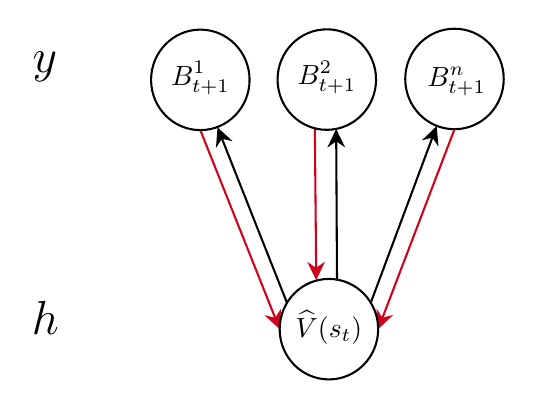
\begin{tikzpicture}[x=0.75pt,y=0.75pt,yscale=-1,xscale=1]
        %uncomment if require: \path (0,300); %set diagram left start at 0, and has height of 300
        
        %Straight Lines [id:da4267952151606098] 
        \draw    (319.82,122) -- (320.2,191.88) ;
        \draw [shift={(319.8,119)}, rotate = 89.69] [fill={rgb, 255:red, 0; green, 0; blue, 0 }  ][line width=0.08]  [draw opacity=0] (8.93,-4.29) -- (0,0) -- (8.93,4.29) -- (5.93,0) -- cycle    ;
        %Straight Lines [id:da6989378371909234] 
        \draw [color={rgb, 255:red, 208; green, 2; blue, 27 }  ,draw opacity=1 ]   (310.17,188.88) -- (309.53,119) ;
        \draw [shift={(310.2,191.88)}, rotate = 269.48] [fill={rgb, 255:red, 208; green, 2; blue, 27 }  ,fill opacity=1 ][line width=0.08]  [draw opacity=0] (8.93,-4.29) -- (0,0) -- (8.93,4.29) -- (5.93,0) -- cycle    ;
        %Shape: Ellipse [id:dp8707618719305075] 
        \draw   (353.08,94.91) .. controls (353.08,81.53) and (363.7,70.7) .. (376.81,70.7) .. controls (389.91,70.7) and (400.53,81.53) .. (400.53,94.91) .. controls (400.53,108.28) and (389.91,119.12) .. (376.81,119.12) .. controls (363.7,119.12) and (353.08,108.28) .. (353.08,94.91) -- cycle ;
        %Straight Lines [id:da13933094112344846] 
        \draw [color={rgb, 255:red, 208; green, 2; blue, 27 }  ,draw opacity=1 ]   (341.1,212.65) -- (376.81,119.12) ;
        \draw [shift={(340.03,215.46)}, rotate = 290.89] [fill={rgb, 255:red, 208; green, 2; blue, 27 }  ,fill opacity=1 ][line width=0.08]  [draw opacity=0] (8.93,-4.29) -- (0,0) -- (8.93,4.29) -- (5.93,0) -- cycle    ;
        %Shape: Ellipse [id:dp9097319337144372] 
        \draw   (291.56,95.2) .. controls (291.56,81.82) and (302.18,70.99) .. (315.29,70.99) .. controls (328.39,70.99) and (339.01,81.82) .. (339.01,95.2) .. controls (339.01,108.57) and (328.39,119.41) .. (315.29,119.41) .. controls (302.18,119.41) and (291.56,108.57) .. (291.56,95.2) -- cycle ;
        %Straight Lines [id:da3769355222150532] 
        \draw [color={rgb, 255:red, 208; green, 2; blue, 27 }  ,draw opacity=1 ]   (291.47,212.67) -- (254.35,119.55) ;
        \draw [shift={(292.58,215.46)}, rotate = 248.27] [fill={rgb, 255:red, 208; green, 2; blue, 27 }  ,fill opacity=1 ][line width=0.08]  [draw opacity=0] (8.93,-4.29) -- (0,0) -- (8.93,4.29) -- (5.93,0) -- cycle    ;
        %Straight Lines [id:da1253267073766362] 
        \draw [color={rgb, 255:red, 0; green, 0; blue, 0 }  ,draw opacity=1 ]   (263.71,120.96) -- (296.02,202.56) ;
        \draw [shift={(262.61,118.17)}, rotate = 68.4] [fill={rgb, 255:red, 0; green, 0; blue, 0 }  ,fill opacity=1 ][line width=0.08]  [draw opacity=0] (8.93,-4.29) -- (0,0) -- (8.93,4.29) -- (5.93,0) -- cycle    ;
        %Shape: Ellipse [id:dp7350394708339132] 
        \draw   (292.58,215.46) .. controls (292.58,202.09) and (303.2,191.25) .. (316.3,191.25) .. controls (329.41,191.25) and (340.03,202.09) .. (340.03,215.46) .. controls (340.03,228.83) and (329.41,239.67) .. (316.3,239.67) .. controls (303.2,239.67) and (292.58,228.83) .. (292.58,215.46) -- cycle ;
        %Shape: Ellipse [id:dp34753658855295044] 
        \draw   (230.62,95.34) .. controls (230.62,81.97) and (241.24,71.13) .. (254.35,71.13) .. controls (267.45,71.13) and (278.07,81.97) .. (278.07,95.34) .. controls (278.07,108.71) and (267.45,119.55) .. (254.35,119.55) .. controls (241.24,119.55) and (230.62,108.71) .. (230.62,95.34) -- cycle ;
        %Straight Lines [id:da6916637423351373] 
        \draw [color={rgb, 255:red, 0; green, 0; blue, 0 }  ,draw opacity=1 ]   (367.15,120.44) -- (336.7,202.13) ;
        \draw [shift={(368.2,117.63)}, rotate = 110.44] [fill={rgb, 255:red, 0; green, 0; blue, 0 }  ,fill opacity=1 ][line width=0.08]  [draw opacity=0] (8.93,-4.29) -- (0,0) -- (8.93,4.29) -- (5.93,0) -- cycle    ;
        
        % Text Node
        \draw (316.33,214.5) node   [align=left] {$\displaystyle \widehat{V}( s_{t})$};
        % Text Node
        \draw (254.43,94.4) node   [align=left] {$\displaystyle B^{1}_{t+1}$};
        % Text Node
        \draw (315.37,94.25) node   [align=left] {$\displaystyle B^{2}_{t+1}$};
        % Text Node
        \draw (377.91,95.99) node   [align=left] {$\displaystyle B^{n}_{t+1}$};
        % Text Node
        \draw (171.67,200.4) node [anchor=north west][inner sep=0.75pt]  [font=\LARGE]  {$h$};
        % Text Node
        \draw (172,80.4) node [anchor=north west][inner sep=0.75pt]  [font=\LARGE]  {$y$};
        
        \end{tikzpicture}
    \end{adjustbox}
\end{center}
\caption[\textbf{Multi-task learning}]{Adapted from \cite{bengio2017deep}. The figure represents how multi-task learning could be used in an ANN to force the the latent representation $h$ to be a sensible approximation of $V(s_t)$. Here $\widehat{V}(s_t)$ indicates the representation generated by a recurrent layer at time $t$ while $B_{t+1}=\{B^n_{t+1}: n \in N\}$ are $N$ targets quantifying the strength of the next interaction (in terms of frequency and amount of behaviour)  between $I$ and $O$. Black and red arrows are respectively the direction of the computations and the flow of the error gradient. Circles indicate computational blocks similar to those in figures \ref{fig: ffnn} and \ref{fig: ffnn_rnn}.}
\label{fig: multi_task}
\end{figure}

\section{Discussion}
\lorem